\begin{figure}
	\centering
	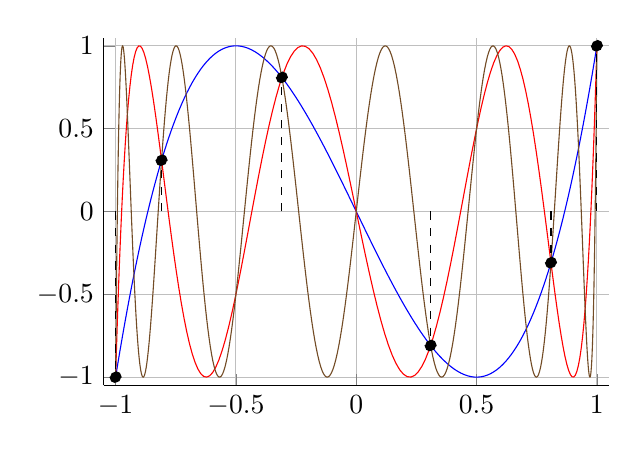
\begin{tikzpicture}
		\begin{axis}[%
			width=8cm, height=6cm,
			axis lines*=left,
			xmin=-1.0, xmax=1.0, ymin=-1.0, ymax=1.0,
			grid=major,
%			xtick = {-1,0,1},
%			ytick = {-1,0,1},
			clip marker paths=false,
			enlargelimits={abs=0.05},
			]%
			\addplot+[samples=200, domain=0:pi, no marks] ({cos(deg(x))}, {cos(3*deg(x))});% T_3
			\addplot+[samples=200, domain=0:pi, no marks] ({cos(deg(x))}, {cos(7*deg(x))});% T_7
			\addplot+[samples=500, domain=0:pi, no marks] ({cos(deg(x))}, {cos(13*deg(x))});% T_13
%			\addplot+[domain=-1:1, no marks, samples=200, black, dotted] {16*x^5 - 20*x^3 + 5*x};% T_5
			\addplot+[samples=6, domain=0:pi, ycomb, dashed, mark=*, black] ({cos(deg(x))}, {cos(3*deg(x))});% noeuds CGL de T_5
		\end{axis}
	\end{tikzpicture}
	\caption{Les polynômes $T_n (\protect\legenddash{mycolor_1})$, $T_{2N - n} (\protect\legenddash{mycolor_2})$ et $T_{2N + n} (\protect\legenddash{mycolor_3})$ sont indiscernables aux n\oe uds CGL de $T_N$ (ici, $n = 3$ et $N = 5$).}
	\label{fig:aliasing_cgl}
\end{figure}